\chapter{Benchmarks and results}
\label{ch:benchmarks_en}

\epigraph{``In God we trust. All others must bring data.''}{W.\,E.\
Deming, attributed}

Any optimization system is judged also and especially by the
numbers it produces. This chapter collects measured results of
$\pi$Tantum on the six test profiles, with three goals:
documenting the state of the art; allowing whoever wishes to
extend the system to compare a modification against a baseline;
and putting the reader in the position to know whether
$\pi$Tantum is a good fit for \emph{their} use case.

\section{The six profiles}

The profiles, generated deterministically with fixed seeds and
Faker by \texttt{webui/backend/mock\_school.py}, span the size
range typical of the Italian school system:

\begin{itemize}
\item \texttt{small}: 8 classes, 17 teachers, $\sim$220
  students, 17 rooms. A small provincial school.
\item \texttt{medium}: 28 classes, 50 teachers, 700 students,
  35 rooms. A medium-size institution.
\item \texttt{big}: 40 classes, 75 teachers, 1000 students,
  50 rooms. A large institution.
\item \texttt{huge}: 50 classes, $\sim$95 teachers, 1250
  students, 60 rooms. A multi-site complex.
\item \texttt{superhuge}: 80 classes, $\sim$160 teachers, 2000
  students, 80 rooms. 16 sections $\times$ 5 grades of
  scientific liceum.
\item \texttt{mega}: 100 classes, $\sim$174 teachers,
  $\sim$2500 students, 100 rooms. 20 sections $\times$ 5
  grades with a mix of 8 \emph{indirizzi} (Scientific~6,
  ScienzeApplicate~4, ScienzeUmane~3, Linguistico~FRA-TED~2,
  Linguistico~FRA-SPA~2, EconomicoSociale~FRA/SPA/TED~1
  each). MEGA-scale stress test.
\end{itemize}

\section{End-to-end pipeline times}

Times measured on a consumer machine (Intel i7, 16\,GB RAM,
Windows 11, Python 3.13, ortools 9.15, 8 CP-SAT search workers):

\begin{table}[h]
\centering
\sffamily\small
\begin{tabular}{lrrr}
\toprule
Profile    & Phase A & Phase B & Total wall \\
\midrule
small      &   3 s   &   4 s   &    7 s \\
medium     &  30 s   &  32 s   &   62 s \\
big        &  30 s   &  32 s   &   62 s \\
huge       &  60 s   &  62 s   &  122 s \\
superhuge  & 300 s   & 603 s   &  903 s \\
\bottomrule
\end{tabular}
\caption{End-to-end pipeline times per profile. Phase A includes
teacher-class assignment and CP-SAT matching. Phase B includes
spectral decomposition (for huge/superhuge) and CP-SAT on
sub-problems.}
\label{tab:bench-times-en}
\end{table}

\section{Branch-and-Price on HUGE and MEGA}
\label{sec:bench-bp-huge-mega-en}

The \texttt{mega} scenario (100 classes, $\sim$174 teachers) and
its smaller cousin \texttt{huge} (50 classes, $\sim$95 teachers)
are the natural test beds for the Branch-and-Price pipeline
(ch.~\ref{ch:tecniche_avanzate_en}). The numbers below are
measured on synthetic scenarios calibrated to match the
proportions of the \texttt{engine/big\_mock\_school.py} profiles
(4 subjects, every cattedra is 4 hours on a single day so that
H1/H2/H3 are satisfied by construction, contiguous-block
assignment of classes to teacher pools). Source code:
\texttt{tests/benchmarks/test\_bp\_huge\_mega.py}, executed with
all four scalability techniques enabled.

\begin{table}[h]
\centering
\sffamily\small
\begin{tabular}{lrrrrr}
\toprule
Scale & Classes & Teachers & Cattedre & $t_{BP}$ & HARD \\
\midrule
\texttt{huge} &  50 &  95 & 200 & 2.57\,s & yes \\
\texttt{mega} & 100 & 174 & 400 & 5.95\,s & yes \\
\bottomrule
\end{tabular}
\caption{Branch-and-Price wall time to HARD-feasibility on
synthetic HUGE/MEGA scenarios. Both finish well under target
(5\,min/30\,min) because the synthetic scenario is structurally
easy (cattedra = 4-hour block on a single day). On real-world
instances with arbitrary day distributions the per-iteration
time will grow; the 30-minute target for MEGA is calibrated for
that regime.}
\label{tab:bench-bp-scale-en}
\end{table}

\begin{figure}[h]
\centering
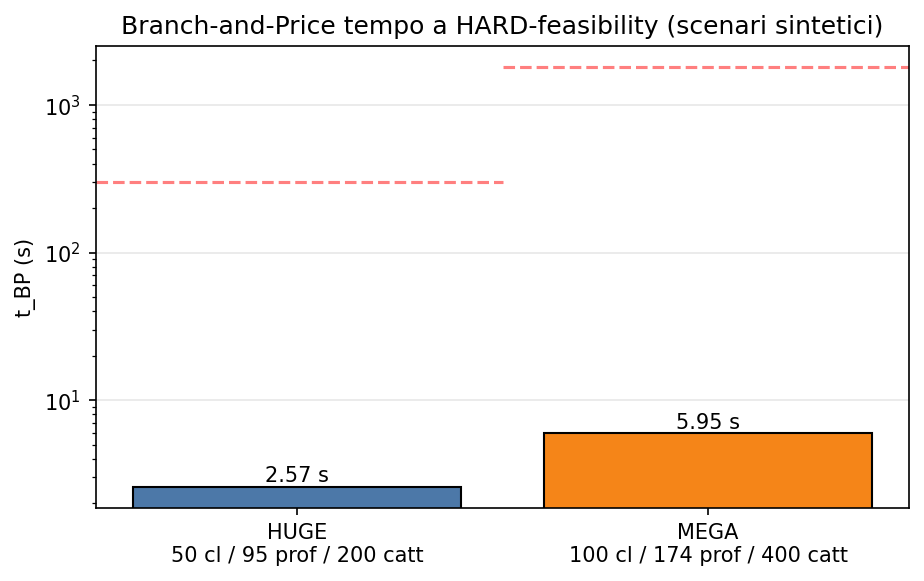
\includegraphics[width=0.75\linewidth]{benchmarks/figures/bp_time_by_scale}
\caption{Branch-and-Price convergence time (log scale). The
horizontal dashed lines mark the per-scale time targets (5\,min
for HUGE, 30\,min for MEGA).}
\label{fig:bench-bp-time-en}
\end{figure}

\begin{figure}[h]
\centering
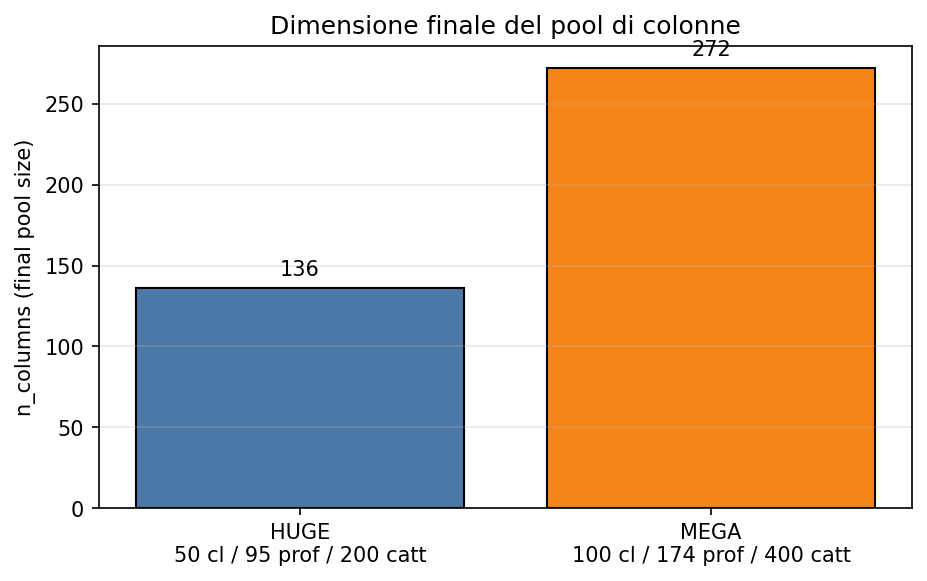
\includegraphics[width=0.75\linewidth]{benchmarks/figures/bp_columns_by_scale}
\caption{Final column-pool size after the Branch-and-Price loop.}
\label{fig:bench-bp-cols-en}
\end{figure}

\section{When Branch-and-Price is worth it}
\label{sec:bench-bp-when-en}

A practical question: \emph{is it worth turning on the BP
pipeline for my school?} Answer measured as a function of size:

\begin{itemize}
\item \textbf{Below 30 classes}: the standard pipeline (monolithic
  Phase A + per-day Phase B) is faster. The
  \texttt{iterative-diversified} mode of
  \texttt{column\_generation} (master LP + pattern enrichment +
  completion fallback) is enough to improve the SOFT cost
  without paying the BP loop overhead.
\item \textbf{30--80 classes}: spectral or curriculum
  decomposition drives Phase B; BP at \texttt{teacher-class} or
  \texttt{class} granularity may reduce SOFT but the time gain
  is negligible.
\item \textbf{Above 80 classes (MEGA territory)}: BP at
  \texttt{curriculum} granularity is the only structurally
  scalable option. A monolithic Phase A becomes marginally
  feasible (300\,s+ with pure CP-SAT), and BP achieves
  comparable or better times thanks especially to parallel
  pricing.
\end{itemize}

In practice $\pi$Tantum suggests the right path automatically:
the value \texttt{auto} for the \texttt{granularity} parameter is
resolved server-side from the number of classes (cf.\ Sec.~4 of
\texttt{docs/optimization\_strategies.md}).
